\section{Report Prioritization}
Before our study, we first preprocess the data set. We delete the data with illogical detection date, such as one data with detection date $4/21/1600$. Additionally, we erase the data whose submission day is earlier than its detection day which is apparently irrational. After the above operations, we get the processed 4411 pieces of data set.
\subsection{General Idea}
When evaluating a sighting report, the first thing that needs to be judged is its amount of information. If its information is lacking then it is very likely to be classified as unverified. Such a report is not worthy of more analysis. Secondly, it needs to be prioritized by judging the possibility of its occurrence based on its existing information including latitude and longitude, detection date, and notes.

Next, according to the latitude and longitude, we can obtain the \textbf{possibility of pests appearing in the area} based on PS-CA model. Besides, we can judge the \textbf{likelihood of pests appearing at this time} from the detection time and pest habits. \textbf{The certainty expressed in the description} extracted from the note is also an important factor. From the image information, \textbf{the similarity between the observed insect and the pest} can be calculated by FCEM-AHP model. 

Then we use a multi-index evaluation method considering these four factors to prioritize the sighting reports. Our model idea is shown in Figure \ref{fig:idea}.
\begin{figure}[H]
    \centering
    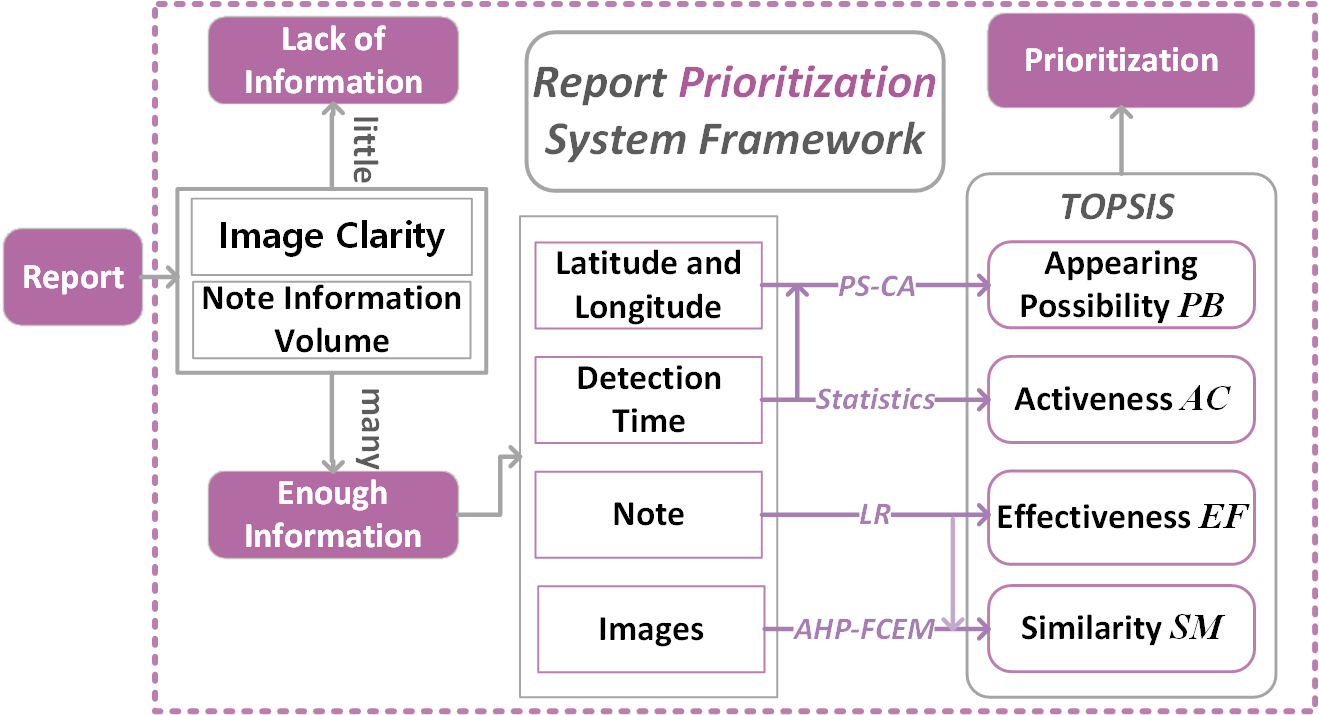
\includegraphics[scale = 0.5]{Chapter-2021C/images-2021C/3-idea.png}
    \caption{Report Prioritization System Framework}
    \label{fig:idea}
\end{figure}

\subsection{Data Screening}

In the sighting report, the most important part is the image. Therefore, image recognition will play an important role in prioritizing reports. In fact, due to the scarcity of correct samples, we cannot train a powerful machine learning system in a limited time. So we changed our thinking and rely on the existing robust insect recognition platform to perform image recognition.

First, we associate the GlobalID of each report with the image file name.

Then we upload the image to a website\cite{insect} with an accuracy of about 78.45\%, which can recognize the image and output the name of the insect in the image. Of course, if the image is blurry or there are no insects in it, it will output ‘no insects’ results.

If the website can not identify the insect in the picture, we assume that the information of this picture is not enough for the judgement and will be placed in a screen-out zone. 

For those reports in the screen-out zone, we calculate the informative score of the given notes by logistic regression to determine whether this certain report will be screened out or not.

To calculate the informative score of the given notes, we need to assign every word appearing in the report with a score to depict its amount of information. As logistic regression is a widely-used algorithm for binary classification, we use logistic regression to judge whether a certain word is informative or not:
\vspace{0.5cm}

\begin{algorithm}[H]
\caption{Logistic Regression}
  \KwIn{Notes set $\mathcal{N}=\{ n_1, n_2, \dots, n_k \}$, Labels set $\mathcal{L}=\{ l_1, l_2, \dots, l_k \}$}  
  \KwOut{Words informative scores $\mathcal{S}$}  
  Construct an ideal score set of all the notes
  
  $\mathcal{SN}_{ideal}=\{ sn_1, sn_2, \dots, sn_k \}$:
  
  \For{$n_i$ \text{in notes set} $\mathcal{N}$}{
   \If{\text{the label} $l_i$ of $n_i$ \text{is Positive or Negative}}{ 
        $sn_i=1$, which means that this note has enough information
    }
    \ElseIf{$l_i$ \text{is Unverified}}{
        $sn_i=0$, which means that this note is lack of information
    }
  }
  Train the words informative scores to minimize the loss function:
  $\mathcal{S}=argmin(\sum_{i=1}^k (sn_i-\frac{1}{1+e^{\sum s\in\mathcal{S}}})^2)$
  
\end{algorithm}

Trained words informative scores are shown in the following word cloud:
\begin{figure}[H]
    \centering
    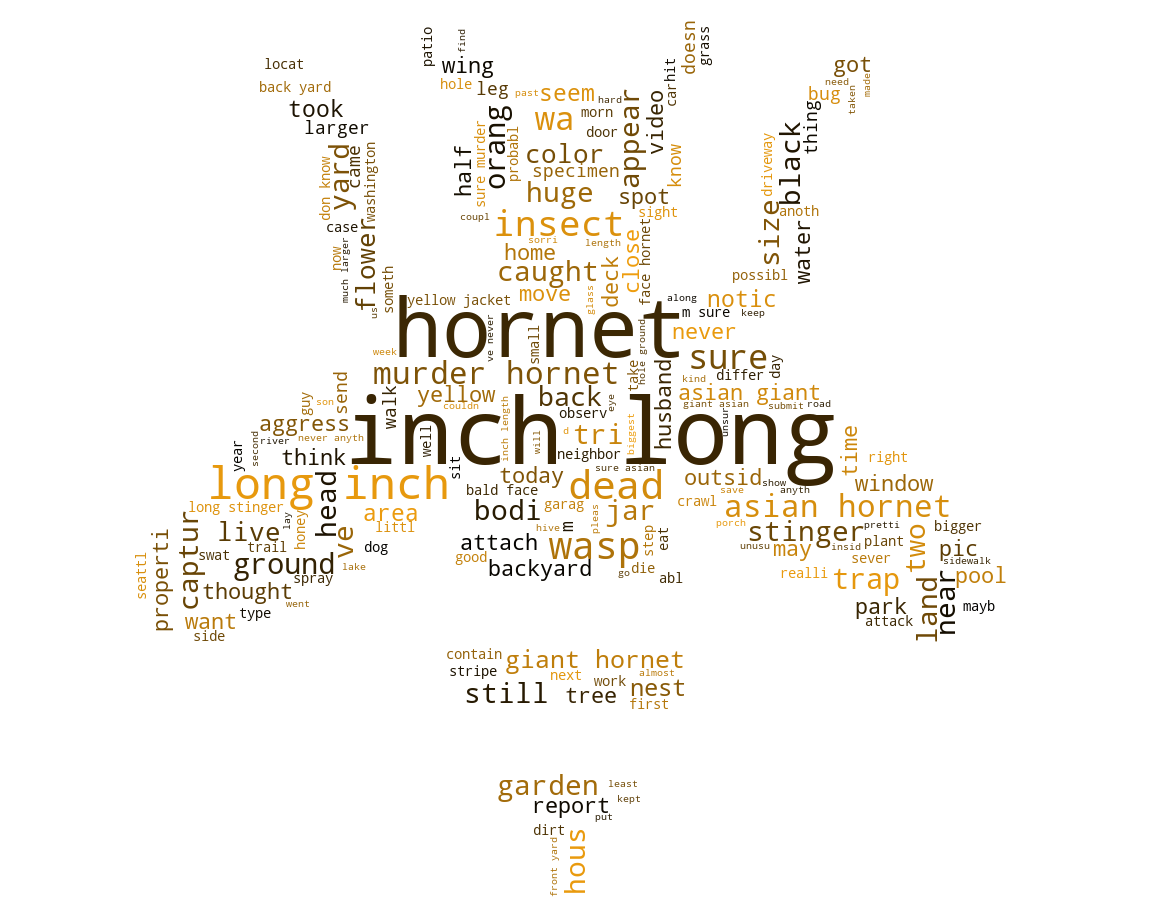
\includegraphics[scale = 0.3]{Chapter-2021C/images-2021C/3-word cloud.png}
    \caption{Word cloud of informative score}
    \label{fig:word cloud}
\end{figure}


Then we use the sigmoid funtion to define the informative score of the whole note. For the note of a new report $rp$, its informative score $S_{rp}$ is defined as:

\begin{equation*}
    S_{rp} = \frac{1}{1+e^{\sum_{i=0}^k s_i}}
\end{equation*}

where $s_i$ represents the informative score of the $i^{th}$ word in this report notes. 

For a report $rp$ in the screen-out zone, (which means that its picture can not be identified by the insect classification website), $rp$ will be screened out in this term if $S_{rp}<0.5$.


\subsection{Report Prioritization based on TOPSIS}
In this section, we use \textbf{Technique for Order Preference by Similarity to an Ideal Solution (TOPSIS)} to prioritize the reports most likely to be positive sightings.

The TOPSIS method \parencite{TOPSIS} is a multiple attribute decision-making method. For example, Zhongyou Xing has studied the introduction of foreign players in CBA games on the application of TOPSIS \parencite{TOPSIS-CBA}.

The TOPSIS method choose several evaluation indices towards the samples, normalize the indices, obtain the best and the worst vector value, calculate the distance between the sample and the best and worst vector, and calculate the relative approach degree.

Finally, the sample is ordered by the value of the relative approach degree.

Continuing the analysis in section 4.1, we define the four influencing factors in details and design strategies to obtain them. These four indices notations is shown in Table \ref{tbl:2021C-Notations of TOPSIS indices.}.

%%三线表 cellular automata notation
\begin{table}[H]
    \renewcommand\arraystretch{2}   %%控制行间距
    \centering
    \caption{Notations of TOPSIS indices.}
    \begin{tabular}{ccc}    %%三列均左对齐
        \toprule  %%表格横线加粗
        \specialrule{0em}{2pt}{2pt}    %%添加透明线控制行高
        Symbol & Definition & Notes \\
        \specialrule{0em}{2pt}{2pt}    %%添加透明线控制行高
        \midrule
        \specialrule{0em}{1pt}{1pt}
        $RP$ & the set of reports & $RP = \{ rp_1, rp_2, \dots, rp_n \}$ \\
        $PB$ & the set of possibility of pest emerging & $PB = \{ pb_1, pb_2, \dots, pb_n \}$ \\
        $AC$ & the set of activeness of pests & $AC = \{ ac_1, ac_2, \dots, ac_n \}$ \\
        $EF$ & the set of note effectiveness of reports & $EF = \{ ef_1, ef_2, \dots, ef_n \}$ \\
        $SM$ & the set of similarity of the reports to pests & $SM = \{sm_1, sm_2, \dots, sm_n \}$ \\
        \specialrule{0em}{1pt}{1pt}
        \bottomrule
    \end{tabular}
    \label{tbl:2021C-Notations of TOPSIS indices.}
\end{table}

In all, a sample report $rp_i$ contains four indices, which can be represented by 
\begin{equation*}
    rp_i = \{ pb_i, ac_i, ef_i, sm_i \}.
\end{equation*}

\begin{enumerate}[\quad\bf 1.]
\item \textbf{Emerging Possibility of the Pest by PS-CA model}%由经纬度获得概率密度

As a result of the \textbf{PS-CA model}, we have the state of every cell $s_{i,t}$ in the cellular automata after the entire simulation. Regarding the meaning of cell state, $s_{i,t}$ represents the degree of the bee gathering of the $i^{th}$ cell at time $t$. 

\begin{figure}[H]
    \centering
    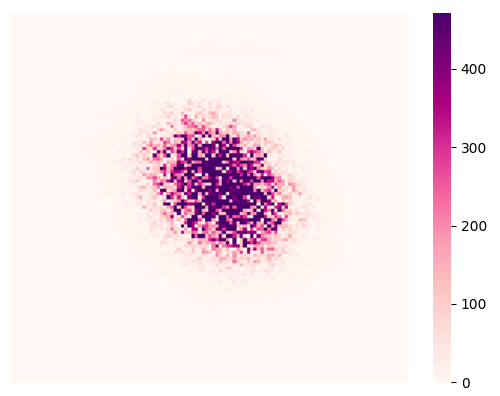
\includegraphics[scale = 0.5]{Chapter-2021C/images-2021C/4-relitu.png}
    \caption{Emerging Possibility of the Pest after one year simulation.}
    \label{fig:2021C-relitu}
\end{figure}

In terms of a sample report $rp_i$, we transfer its detection time to the simulation time $t$. Next, we calculate the cell number $j$ with the longitude and latitude of the report. Consequently, we get the state $s_{j,t}$. Finally, we divide it by the maximum state of all cells to obtain the index $pb_i = \frac{s_{j,t}}{\max \{ s_{k,t} \}}, k=(1, 2, \dots, n)$. Figure \ref{fig:2021C-relitu} shows our results for one year simulation.

\item \textbf{Activeness of the Pest by time}%定义各月份活跃度
%%可以补reference

From the introduction of the pest, we know that pests are only seen outside the nest from spring to hibernation\parencite{NPRG}. It can imply that pests' activeness differs on the basis of time. We define the activeness to be 1 from May to December, and 0.5 otherwise.

Regarding a sample report $rp_i$, we get the $month$ from its detection time and have the activeness $ac_i$ through

\begin{equation*}
    ac_i = \begin{cases}
    1 &, \text{month}=5, 6, 7, 8, 9, 10, 11, 12; \\
    0.5 &, \text{otherwise}.
    \end{cases}
\end{equation*}

\item \textbf{Note Effectiveness}

Similar to what we have done in Section 4.2 Data Screening, we train the informative score of all the words appearing in the reports and calculate a total informative score of every piece of note using the sigmoid function. For the note of a new report $rp$, its informative score $S_{rp}$ is defined as:
\begin{equation*}
    ef_{rp} = S_{rp} = \frac{1}{1+e^{\sum_{i=0}^k s_i}}
\end{equation*}

where $s_i$ represents the informative score of the $i^{th}$ word in this report notes. 

However, there is some difference between this part and the informative scores training in Section 4.2. In Section 4.2, labels of the trained notes are 'Have enough information' and 'Lack of information', while in this part, labels are 'Positive' and 'Negative'. The former aims to tell the difference between informative notes and those that are not, while the latter distinguish the Positive ID from the Negative.


\item \textbf{Possibility of misclassification of image recognition}

With the help of the insect recognition website\cite{insect}, we can get the general class of the insect in the pictures by using a simple script to upload them and read the results on the website. Then, we can obtain the similarity between the insect and the pest based on the recognition result and the FCEM-AHP model. The reason for using similarity as an evaluation index instead of directly relying on insect recognition websites is that recognition has uncontrollable errors, and we can reduce errors as much as possible by combining the results with similarity as an index.
 
For example, we randomly select a report with a GlobalID of {2CE88ACB-6B4B-4357-91F1-813D079B5057}, and the attached image name is ATT154\_20200512\_180734. The result of the image being identified on the website is a yellow jacket. The similarity between yellowjacket and the pests studied by us is 59.57\%, so its $sm$ value is 0.5957.

%Based on the AHP-FCEM model in section 3, we can finally get a value $v_i$, which we denotes as the similarity. As for a sample report $rp_i$, we follow the rules of the AHP-FCEM model to get the value. By artificially examining the picture and note of the report, we fill in the value of five factors $FV^i$ according to the definition of the AHP-FCEM model and calculate the value $v_i$. Then we simply get the similarity $sm_i$ by $sm_i = v_i$.

\end{enumerate}

After obtaining all the values of the indices, we run the TOPSIS method to prioritize the top-ranked reports, which we regard as most likely to be positive sightings.

But theoretical reasoning is not enough. We randomly selected two positive reports, two negetive reports, two unverified reports and 14 unprocessed reports from the report set for testing. Their numbers are 1, 2, \dots , 20. Their processing and calculation procedures are shown in Figure \ref{fig:result of the prioritization system}.
\begin{figure}[H]
    \centering
    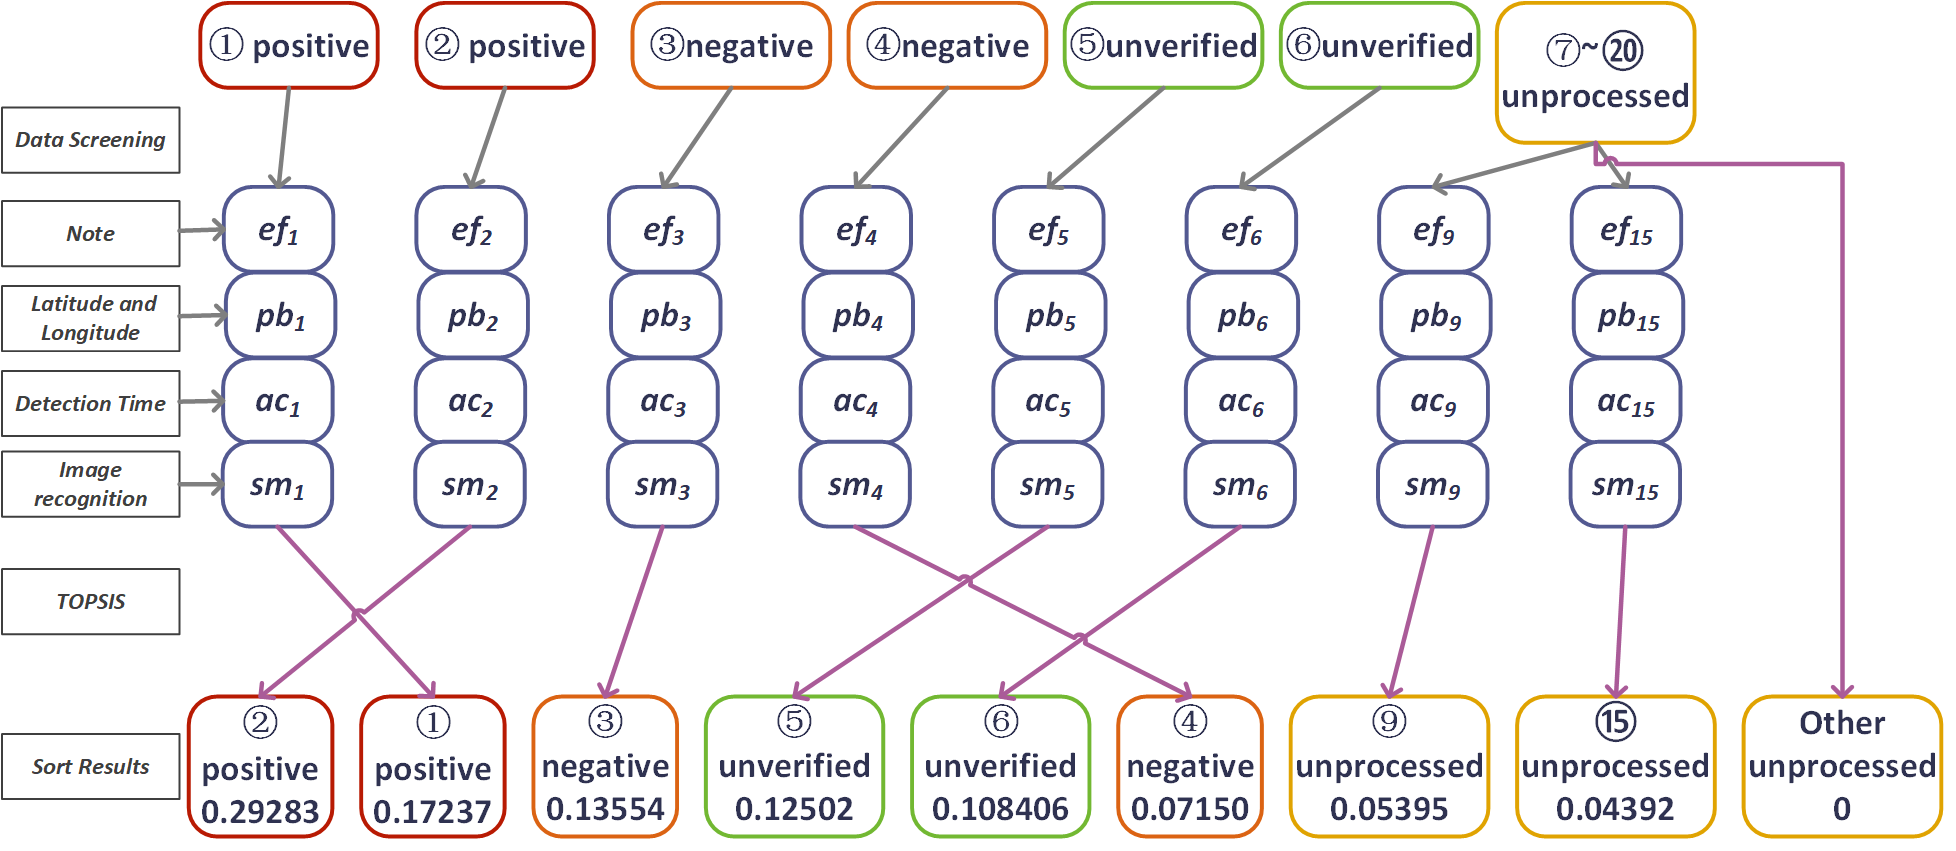
\includegraphics[scale = 0.4]{Chapter-2021C/images-2021C/3-result.png}
    \caption{The test result of the prioritization system (the priority decreases from left to right).}
    \label{fig:result of the prioritization system}
\end{figure}

This test result is in line with expectations and reality. Both positive reports are ranked at the forefront, which shows that our prioritization system is effective.

\vspace{1cm}